\documentclass[11pt]{article}
\usepackage{worksheet_style}

%\worksheetfilledtrue
\begin{document}
\worksheetheader{25}{Surface Integrals}

\begin{background}
We've integrated functions along curves (line integrals) and over flat regions (double integrals). Today we integrate over curved surfaces in 3D. Surface integrals compute mass of a shell, and flux integrals measure how much a vector field flows through a surface. These are the ingredients we need for Stokes' and the Divergence Theorem.
\end{background}

\wsection{Parametric Surfaces}

\begin{defbox}{Parametric Surface}
A \textbf{parametric surface} $S$ is the image of a continuous map $\vect{r}:D\to\R^3$, where $D\subseteq\R^2$. Each pair $(u,v)\in D$ is sent to a point on $S$ — think of latitude and longitude on a globe.
\[\vect{r}(u,v) = \vec{x(u,v),\; y(u,v),\; z(u,v)}, \qquad (u,v)\in D.\]

-- \textbf{Tangent vectors:} $\vect{r}_u = \dfrac{\partial\vect{r}}{\partial u}$, \; $\vect{r}_v = \dfrac{\partial\vect{r}}{\partial v}$

-- \textbf{Normal vector:} $\vect{n} = \vect{r}_u \times \vect{r}_v$ \; (perpendicular to $S$; nonzero where $S$ is smooth)

-- \textbf{Surface area element:} $dS = \|\vect{r}_u \times \vect{r}_v\|\,du\,dv$
\end{defbox}

\wsubsection{Common Parameterizations}

\begin{center}
\footnotesize
\renewcommand{\arraystretch}{1.55}
\begin{tabular}{@{}llll@{}}
\toprule
\textbf{Surface} & \textbf{Parameterization $\vect{r}(u,v)$} & \textbf{Domain} & \textbf{$dS=\|\vect{r}_u\times\vect{r}_v\|\,du\,dv$} \\
\midrule
Graph $z=g(x,y)$ & $\vec{x,\; y,\; g(x,y)}$ & $(x,y)\in D$ & $\sqrt{1+g_x^2+g_y^2}\,dA$ \\
Sphere $x^2+y^2+z^2=a^2$ & $\vec{a\sin\phi\cos\theta,\; a\sin\phi\sin\theta,\; a\cos\phi}$ & $\theta\in[0,2\pi],\ \phi\in[0,\pi]$ & $a^2\sin\phi\,d\phi\,d\theta$ \\
Cylinder $x^2+y^2=R^2$ & $\vec{R\cos\theta,\; R\sin\theta,\; z}$ & $\theta\in[0,2\pi],\ z\in[c,d]$ & $R\,d\theta\,dz$ \\
Cone $z=\sqrt{x^2+y^2}$ & $\vec{r\cos\theta,\; r\sin\theta,\; r}$ & $\theta\in[0,2\pi],\ r\in[0,h]$ & $r\sqrt{2}\,dr\,d\theta$ \\
Plane thru $P_0$, dirs $\vect{a},\vect{b}$ & $P_0 + s\vect{a}+t\vect{b}$ & $(s,t)\in D$ & $\|\vect{a}\times\vect{b}\|\,ds\,dt$ \\
Rev.\ of $y=f(x)$ about $x$-axis & $\vec{x,\; f(x)\cos\theta,\; f(x)\sin\theta}$ & $x\in[a,b],\ \theta\in[0,2\pi]$ & $|f(x)|\sqrt{1+f'(x)^2}\,dx\,d\theta$ \\
\bottomrule
\end{tabular}
\end{center}

\begin{formulabox}{Special Case: $z = g(x,y)$}
\[dS = \wbml{\sqrt{1 + g_x^2 + g_y^2}\,dA}\]
\[\vect{n}\,dS = \vec{-g_x,\; -g_y,\; 1}\,dA \quad \text{(upward-pointing normal)}\]
For downward normal, negate: $\vec{g_x,\; g_y,\; -1}\,dA$.
\end{formulabox}

\wsection{Scalar Surface Integrals}

\begin{defbox}{Surface Integral of a Scalar Function}
The \textbf{surface integral} $\iint_S f\,dS$ generalizes the double integral from a flat 2D region to a curved surface in $\R^3$. It sums values of $f$ over $S$ weighted by the true area element $dS$.
\[\iint_S f\,dS = \wbml{\iint_D f(\vect{r}(u,v))\;\|\vect{r}_u \times \vect{r}_v\|\,du\,dv}\]
For $z = g(x,y)$:
\[\iint_S f\,dS = \iint_D f(x,y,g(x,y))\,\sqrt{1 + g_x^2 + g_y^2}\,dA\]

-- \textbf{Applications:} mass ($f = \rho$), average value on a surface
\end{defbox}

\begin{formulabox}{Special Case: $f \equiv 1$ gives Surface Area}
Setting $f = 1$ in the surface integral turns it into the \textbf{surface area} of $S$:
\[\text{Area}(S) \;=\; \iint_S 1\,dS \;=\; \wbml{\iint_D \|\vect{r}_u \times \vect{r}_v\|\,du\,dv}\]
For a graph $z = g(x,y)$ over a region $D$ in the $xy$-plane:
\[\text{Area}(S) \;=\; \iint_D \sqrt{1 + g_x^2 + g_y^2}\,dA\]
\end{formulabox}

\begin{example}[Mass of a Hemispherical Shell]
Find the mass of the upper hemisphere $x^2+y^2+z^2 = 9$, $z \ge 0$, with density $\rho = z$.

\wbbox{
1. \textbf{Parameterize:} $\vect{r}(\theta,\phi) = \vec{3\sin\phi\cos\theta,\; 3\sin\phi\sin\theta,\; 3\cos\phi}$

\quad $\theta \in [0,2\pi]$, $\phi \in [0,\pi/2]$; \quad $\|\vect{r}_\theta \times \vect{r}_\phi\| = 9\sin\phi$

2. \textbf{Set up:} $\rho = z = 3\cos\phi$

$M = \ds\int_0^{2\pi}\int_0^{\pi/2}(3\cos\phi)(9\sin\phi)\,d\phi\,d\theta$

3. \textbf{Evaluate:}
$= 27\int_0^{2\pi}d\theta \int_0^{\pi/2}\sin\phi\cos\phi\,d\phi = 27 \cdot 2\pi \cdot \dfrac{1}{2} = \boxed{27\pi}$
}{5cm}
\end{example}

\wsection{Flux Integrals}

\begin{defbox}{Flux of a Vector Field Through a Surface}
The \textbf{flux} of a vector field $\vect{F}$ across an oriented surface $S$ measures the net rate at which $\vect{F}$ crosses $S$ in the direction of the chosen unit normal $\uvec{n}$. If $\vect{F}$ is a fluid velocity field, the flux is the volume of fluid passing through $S$ per unit time.
\[\iint_S \vect{F}\cdot d\vect{S} = \wbml{\iint_D \vect{F}(\vect{r}(u,v))\cdot(\vect{r}_u \times \vect{r}_v)\,du\,dv}\]

For $z = g(x,y)$ with \textbf{upward} normal:
\[\iint_S \vect{F}\cdot d\vect{S} = \iint_D \left(-P\,g_x - Q\,g_y + R\right)dA\]

-- \textbf{Interpretation:} \wbi{net flow of $\vect{F}$ through the surface per unit time}{7cm}

-- Positive flux = net flow in direction of chosen normal

-- \textbf{Orientation matters:} flipping normal negates the flux
\end{defbox}

\begin{center}
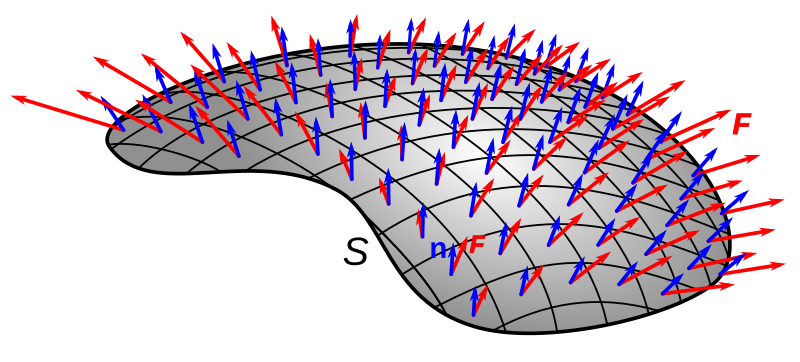
\includegraphics[width=9cm]{pics/surf_int.png}\\
{\small Surface $S$ with normal vectors $\vect{n}$ (blue) and vector field $\vect{F}$ (red). The flux integral measures how much $\vect{F}$ flows through $S$.}
\end{center}

\begin{example}[Flux Through a Paraboloid]
Find the flux of $\vect{F} = \vec{y,\, x,\, z}$ through the paraboloid $z = 1 - x^2 - y^2$, $z \ge 0$, with upward normal.

\wbbox{
1. \textbf{Set up:} $g(x,y) = 1 - x^2 - y^2$, so $g_x = -2x$, $g_y = -2y$

\quad $P = y$, $Q = x$, $R = z = 1 - x^2 - y^2$

\quad Domain $D$: $x^2 + y^2 \le 1$ (disk of radius 1)

2. \textbf{Apply flux formula:}
\begin{align*}
\text{Flux} &= \iint_D(-y(-2x) - x(-2y) + (1-x^2-y^2))\,dA \\
&= \iint_D(2xy + 2xy + 1 - x^2 - y^2)\,dA \\
&= \iint_D(4xy + 1 - x^2 - y^2)\,dA
\end{align*}

3. \textbf{Polar coordinates:} $\ds\int_0^{2\pi}\!\int_0^1(4r^2\cos\theta\sin\theta + 1 - r^2)\,r\,dr\,d\theta$

\quad The $4r^2\cos\theta\sin\theta$ term integrates to 0 over $[0,2\pi]$.

\quad $= \ds\int_0^{2\pi}\!\int_0^1(r - r^3)\,dr\,d\theta = 2\pi\left[\frac{r^2}{2}-\frac{r^4}{4}\right]_0^1 = 2\pi \cdot \frac{1}{4} = \boxed{\frac{\pi}{2}}$
}{7cm}
\end{example}

\begin{example}[Flux Through a Sphere]
Find the outward flux of $\vect{F} = \vec{x,\, y,\, z}$ through the sphere $x^2+y^2+z^2 = a^2$.

\wbbox{
1. \textbf{Outward unit normal:} On the sphere, $\hat{\vect{n}} = \dfrac{1}{a}\vec{x,y,z}$

2. \textbf{Dot product:} $\vect{F}\cdot\hat{\vect{n}} = \dfrac{x^2+y^2+z^2}{a} = \dfrac{a^2}{a} = a$

3. \textbf{Integrate:} $\ds\iint_S \vect{F}\cdot d\vect{S} = \iint_S a\,dS = a \cdot 4\pi a^2 = \boxed{4\pi a^3}$
}{4cm}
\end{example}

\begin{practice}

\prob
Find the surface area of the plane $z = 3 - x - y$ over the triangle $0 \le x \le 1$, $0 \le y \le 1-x$.

\wans{$\wbm{\dfrac{\sqrt{3}}{2}}$}

\vspace{3cm}

\prob
Find the flux of $\vect{F} = \vec{0, 0, 1}$ upward through $z = 1 - x^2 - y^2$ above $z = 0$.

\wans{$\wbm{\pi}$}

\vspace{3cm}

\prob
Compute $\ds\iint_S z\,dS$ where $S$ is the cone $z = \sqrt{x^2+y^2}$, $0 \le z \le 2$.

(\textit{Hint: } $g_x = x/\sqrt{x^2+y^2}$, $g_y = y/\sqrt{x^2+y^2}$, so $\sqrt{1+g_x^2+g_y^2} = \sqrt{2}$.)

\wans{$\wbml{\sqrt{2}\int_0^{2\pi}\!\int_0^2 r \cdot r\,dr\,d\theta = \sqrt{2}\cdot 2\pi \cdot \frac{8}{3} = \frac{16\sqrt{2}\,\pi}{3}}$}

\vspace{4cm}

\prob
Find the flux of $\vect{F} = \vec{x^2, y^2, z^2}$ outward through the unit sphere $x^2+y^2+z^2=1$.

(\textit{Hint: on the unit sphere the outward unit normal is $\uvec{n}=\vec{x,y,z}$, so $\vect{F}\cdot\uvec{n}=x^3+y^3+z^3$. Use symmetry.})

\wans{$\wbm{0}$ \; ($\vect{F}\cdot\uvec{n}=x^3+y^3+z^3$; each term is odd in one variable on a symmetric sphere)}

\vspace{4cm}

\prob
Find the flux of $\vect{F} = \vec{z, x, y}$ upward through the triangle cut from the plane $x + y + z = 1$ in the first octant.

\wans{$\wbml{-P g_x - Q g_y + R = -z(-1) - x(-1) + y = z + x + y = 1; \quad \text{Flux} = \iint_D 1\,dA = \frac{1}{2}}$}

\vspace{3.5cm}

\end{practice}

\end{document}
